\documentclass[aspectratio=169]{beamer} % 16:9 widescreen
\usepackage[utf8]{inputenc}

% --- Estilos del club ---
\usepackage{config/pumasmas}
% --- Complexity Analysis ---
\newcommand{\bigO}[1]{\mathcal{O}(#1)}
\newcommand{\softO}[1]{\tilde{\mathcal{O}}(#1)}
\newcommand{\omegaO}[1]{\Omega(#1)}
\newcommand{\thetaO}[1]{\Theta(#1)}
\newcommand{\smallo}[1]{o(#1)}

% --- Mathematical Sets ---
\newcommand{\RR}{\mathbb{R}}
\newcommand{\ZZ}{\mathbb{Z}}
\newcommand{\NN}{\mathbb{N}}
\newcommand{\QQ}{\mathbb{Q}}

% --- Algorithmic Notations ---
\newcommand{\state}[1]{\text{state}(#1)}
\newcommand{\dpstate}[1]{\text{dp}[#1]}
\newcommand{\cost}[1]{\text{cost}(#1)}
\newcommand{\dist}[1]{\text{dist}(#1)}

% --- Number Theory ---
\newcommand{\floor}[1]{\left\lfloor #1 \right\rfloor}
\newcommand{\ceil}[1]{\left\lceil #1 \right\rceil}
\newcommand{\divisor}{\mid}
\newcommand{\ndivisor}{\nmid}
\newcommand{\modm}[1]{\pmod{#1}}
\newcommand{\congmod}[3]{#1 \equiv #2 \pmod{#3}}
\newcommand{\gcdop}[2]{\text{gcd}(#1, #2)}
\newcommand{\lcmop}[2]{\text{lcm}(#1, #2)}
\newcommand{\eulerphi}[1]{\phi(#1)}
\newcommand{\mobius}[1]{\mu(#1)}
\newcommand{\nCr}[2]{\binom{#1}{#2}}
\newcommand{\nPr}[2]{P_{#2}^{#1}}

% --- Formatting Shorthands ---
\newcommand{\boldtopic}[1]{\textbf{#1}}
\newcommand{\important}[1]{\textcolor{cp-accent}{\textbf{#1}}}
\newcommand{\inlinecode}[1]{\texttt{#1}}

% --- Problem Tags ---
\newcommand{\tagcp}[1]{\hfill \fbox{\small\texttt{#1}}}

% Helper for practice problem links
\newcommand{\practiceproblemlink}[1]{%
    \ifblank{#1}{%
        \textcolor{cp-gray}{\textit{Link no disponible}}%
    }{%
        \scalebox{0.65}{\qrcode{#1}}%
    }%
}

% --- Practice Problems ---
% Usage: \practiceproblem{Name}{Difficulty}{Judge}{Link}
\newcommand{\practiceproblem}[4]{%
    \item \textbf{#1} \hfill \difficultybadge{#2} \\
    \textit{Judge: #3} \hfill \practiceproblemlink{#4}
}

% --- Graph Theory Helpers ---
\newcommand{\tree}[1]{T_{#1}}
\newcommand{\graph}[1]{G_{#1}}
\newcommand{\nodes}{V}
\newcommand{\edges}{E}


% --- Two-column code input ---
% Uso: \twocolumnminted{archivo}{lenguaje}{última línea columna 1}
\newcommand{\twocolumnminted}[3]{%
  \begingroup
    \newcount\startline
    \startline=#3
    \advance\startline by 1
    \begin{columns}
      \begin{column}{0.48\textwidth}
        \inputminted[firstline=1,lastline=#3,linenos,fontsize=\tiny,numbersep=3pt,breaklines]{#2}{#1}
      \end{column}
      \begin{column}{0.48\textwidth}
        \inputminted[firstline=\the\startline,linenos,fontsize=\tiny,numbersep=3pt,breaklines]{#2}{#1}
      \end{column}
    \end{columns}
  \endgroup
}

% --- Custom title page template ---
\setbeamertemplate{title page}{%
  \begin{center}
    % Logo at top right, slightly smaller
    %\hfill
\includegraphics[height=2.0cm]{logo.png}\hspace*{0.5cm}\\[0.8cm]
    \vspace{3.3cm}

    % Title block raised a bit
    \vspace{-0.5cm} % shift upward
    {\Huge\bfseries\color{white}\inserttitle\par}
    \vspace{5mm}
    {\Large\itshape\color{white}Por: \insertauthor\par}
    \vspace{2mm}
    {\normalsize\color{white}Club de Programación Competitiva Pu++\par}
    \vspace{8mm}
    {\large\color{white}\insertdate\par}
  \end{center}
}

% --- Cover slide with custom background ---
\newcommand{\portadapumasmas}[0]%
{
\usebackgroundtemplate{%
  \begin{tikzpicture}[remember picture,overlay]

    % Gradient background
    \path[shade, left color=cover-left, right color=cover-right]
      (current page.south west) rectangle (current page.north east);

    % Large translucent accents
    \fill[white,opacity=0.05,rotate=25]
      (current page.center) circle (7cm);

    \fill[white,opacity=0.03,rotate=-15]
      (current page.north east) circle (5cm);

    % Angled bars
    \fill[cover-left!50!black,opacity=0.2]
      (current page.south west) -- ++(5,0) -- ++(2,2) -- ++(-5,0) -- cycle;

    \fill[cover-right!50!black,opacity=0.2]
      (current page.north east) -- ++(-5,0) -- ++(-2,-2) -- ++(5,0) -- cycle;

    % Subtle scattered circles
    \foreach \i in {1,...,20}{
      \fill[white,opacity=0.04] 
        (rand*14-7, rand*10-5) circle (rand*0.3);
    }

  \end{tikzpicture}%
}
\begin{frame}[plain,noframenumbering] % no slide number on cover
  \titlepage
\end{frame}
}


% --- Metadatos ---
\title{Plantilla de Diapositivas Pu++}
\author{SqueletoCosmico y José Antonio Zarco}
\date{\today}

\begin{document}

% --- Portada ---
\portadapumasmas
\usebackgroundtemplate{}

% --- Tabla de contenidos ---
\begin{frame}{Contenido}
	\tableofcontents
\end{frame}

% --- Secciones ---
% Usa \include{sections/nombre_archivo} para modularizar.

\section{Guía de Uso del Template}
\label{sec:usage_guide}

% --- Intro ---
\begin{frame}{Guía de Uso del Template}
    Esta sección unifica la documentación de funcionalidades y la estructura
    sugerida para nuevos temas.
\end{frame}

% --- Sub-secciones ---
% Cada archivo modular se incluye dentro de un frame o varios frames.
% Puedes decidir si cada archivo genera varias diapositivas o una sola.

\subsection{Introducción}

\begin{frame}{Introducción}
    Este documento sirve como plantilla para \textbf{diapositivas de algoritmia
    competitiva (Pu++)}. 

    El objetivo es mantener un formato consistente, limpio y fácil de leer para
    el material educativo.

    \vspace{0.5cm}

    Para crear una nueva sección, se recomienda:
    \begin{itemize}
        \item Copiar la estructura de esta guía o usar los archivos base como referencia.
        \item Dividir el contenido en subsecciones lógicas:
        \begin{itemize}
            \item \textbf{Teoría}
            \item \textbf{Implementación}
            \item \textbf{Problemas}
        \end{itemize}
    \end{itemize}
\end{frame}


\subsection{Entornos Personalizados}

% --- Intro ---
\begin{frame}{Entornos Personalizados}
    El template incluye varios entornos predefinidos para estructurar las
    diapositivas de forma clara y visual.
\end{frame}

% --- Definiciones y Teoremas ---
\begin{frame}{Definiciones y Teoremas}
    \begin{DefinitionP}[title=Definición Formal]
        Utiliza este entorno para introducir formalmente nuevos conceptos,
        estructuras de datos o términos clave. El argumento opcional
        \texttt{title} permite dar un nombre descriptivo a la definición.
    \end{DefinitionP}

    \begin{TheoremP}[title=Propiedad Matemática]
        El entorno \texttt{TheoremP} sirve para destacar propiedades matemáticas
        fundamentales, lemas o teoremas que justifican la corrección o
        complejidad de un algoritmo.
    \end{TheoremP}
\end{frame}

% --- Consejos y Advertencias ---
\begin{frame}{Consejos y Advertencias}
    \begin{TipP}
        Este entorno se usa para dar consejos o recomendaciones prácticas que
        no son necesariamente reglas estrictas, pero ayudan a resolver
        problemas de manera más eficiente.
    \end{TipP}

    \begin{AlertP}
        Úsalo para advertir sobre errores comunes, desbordamientos de enteros
        (overflow), casos borde complicados o complejidad temporal excesiva.
    \end{AlertP}
\end{frame}

% --- Ejemplos ---
%% NOTA: [fragile] es necesario para incluir verbatim
\begin{frame}[fragile]{Ejemplos}
    \begin{ExampleP}[title=Caso de Prueba]
        Este cuadro es ideal para mostrar ejemplos concretos, como casos de
        entrada y salida, trazas de ejecución paso a paso, o diagramas
        explicativos.
        
        \textbf{Input:}
        \begin{verbatim}
        5
        1 2 3 4 5
        \end{verbatim}

        \textbf{Output:}
        \begin{verbatim}
        15
        \end{verbatim}
    \end{ExampleP}
\end{frame}

\subsection{Código Fuente}

% --- Intro ---
\begin{frame}{Código Fuente}
    El código se resalta automáticamente usando \texttt{minted}.
\end{frame}

% --- Buenas Prácticas ---
\begin{frame}{Buenas Prácticas}
    \begin{TipP}
        \textbf{Recomendación:} Se recomienda mantener el código en archivos
        \texttt{.cpp} separados dentro de la carpeta \texttt{code/} y usar
        \texttt{\textbackslash twocolumnminted} para incluirlos. Esto asegura que
        el código sea compilable y testeable independientemente del documento.
    \end{TipP}
\end{frame}



% --- Ejemplo con archivo externo ---
%% NOTA: [fragile] es necesario para meter código (minted/verbatim)
\begin{frame}[fragile]{Ejemplo: Archivo externo}
    Ejemplo incluyendo el archivo \texttt{code/template.cpp} directamente:

    % Inserta el archivo code/template.cpp 
    \twocolumnminted{code/template.cpp}{cpp}{20}
\end{frame}

% --- Ejemplo con snippet inline ---
%% NOTA: [fragile] es necesario para meter código (minted/verbatim)
\begin{frame}[fragile]{Ejemplo: Código inline}
    También es posible escribir código directamente en el archivo \texttt{.tex} usando el entorno \texttt{minted}, útil para snippets cortos:

    \begin{minted}{cpp}
    // Ejemplo de código inline
    void solve() {
        int n; cin >> n;
        cout << n * 2 << endl;
    }
    \end{minted}
\end{frame}

\subsection{Matemáticas}

\begin{frame}{Matemáticas en la Plantilla}
    Podemos usar comandos personalizados definidos en \texttt{macros.tex} 
    para simplificar la notación común en algoritmia:

    \vspace{0.5cm}

    \begin{itemize}
        \item \textbf{Complejidad:} $\bigO{N \log N}$, $\softO{N}$, $\Omega(N)$
        \item \textbf{Conjuntos Numéricos:} $\RR$ (Reales), $\ZZ$ (Enteros), $\NN$ (Naturales)
        \item \textbf{Combinatoria:} $\nCr{n}{k}$ para coeficientes binomiales
        \item \textbf{Teoría de Números:} $\gcdop{a}{b}$, $\lcmop{a}{b}$, $a \mid b$
        \item \textbf{Otros:} $\floor{x}$, $\ceil{x}$
    \end{itemize}
\end{frame}

\subsection{Problemas de Práctica}

% --- Intro ---
\begin{frame}{Problemas de Práctica}
    Es fundamental incluir una lista de problemas para reforzar el tema. 
    El comando \texttt{\textbackslash practiceproblem} facilita este formato estandarizado.

    \vspace{0.3cm}
    \textbf{Argumentos:} \texttt{\{Nombre\}\{Dificultad\}\{Juez\}\{Link\}}
\end{frame}

% --- Lista de problemas ---
\begin{frame}{Lista de Problemas}
    \begin{itemize}
        \practiceproblem{Sum of Two Values}{Easy}{CSES}{https://cses.fi/problemset/task/1640}
        \practiceproblem{Maximum Subarray Sum}{Medium}{CSES}{https://cses.fi/problemset/task/1643}
        \practiceproblem{Counting Tilings}{Hard}{CSES}{https://cses.fi/problemset/task/2181}
    \end{itemize}
\end{frame}

\begin{frame}{Lista de Problemas}
    \begin{itemize}
        \practiceproblem{Hamiltonian Flights}{Very Hard}{CSES}{https://cses.fi/problemset/task/1690}
        \practiceproblem{Problema Personalizado}{Unknown}{Local}{}
    \end{itemize}
\end{frame}


\subsection{Busqueda binaria sobre la respuesta}

\begin{frame}[plain]
	\centering
	\color{theme-brand-color}
	\Huge \textbf{Busqueda binaria sobre la respuesta}
\end{frame}

\begin{frame}{Busqueda binaria sobre la respuesta}
	La busqueda binaria no es solo un algoritmo de busqueda, sino que
	es la idea de dividir en dos nuestro espacio de busqueda, donde dicho espacio de busqueda
	no solo se refiere a una estructura como un arreglo ordenado, sino a cualquier función monotona.
\end{frame}

\begin{frame}{Funciones monótonas}
	\begin{TheoremP}[title=Función monotonamente creciente]
		Sea f una función tal que $f: \mathbb{R} \rightarrow \mathbb{R}$. Se dice que f es monótonamente creciente si para toda
		$x, y \in \mathbb{R}$ tal que $x < y$ tenemos que $f(x) \leq f(y)$
	\end{TheoremP}

	\begin{figure}[htbp]
		\centering
		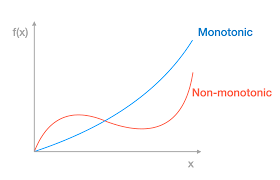
\includegraphics[width=0.5\textwidth]{assets/binary_search_on_the_answer/funcion_monotona_1.png}
	\end{figure}
\end{frame}

\begin{frame}{Funciones monótonas}
	\begin{TheoremP}[title=Función monotonamente decreciente]
		Sea f una función tal que $f: \mathbb{R} \rightarrow \mathbb{R}$. Se dice que f es monótonamente decreciente si para toda
		$x, y \in \mathbb{R}$ tal que $x < y$ tenemos que $f(x) \geq f(y)$
	\end{TheoremP}

	\begin{figure}[htbp]
		\centering
		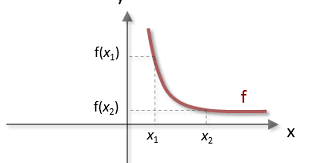
\includegraphics[width=0.5\textwidth]{assets/binary_search_on_the_answer/funcion_monotona_2.png}
	\end{figure}
\end{frame}

\begin{frame}{Busqueda binaria sobre la respuesta}
	Si tenemos un dominio o intervalo de posibles valores en los que se puede encontrar nuestra respuesta,
	entonces podemos hacer busqueda binaria para encontrarla, pero solo si nuestro espacio de busqueda tiene la forma
	de una función monótona.

	\vspace{0.5cm}

	Cada vez que saquemos la mitad de nuestro intervalo, digamos que es el valor $m$, vamos a pobrar si dicha posible respuesta $m$
	soluciona nuestro problema, y dependiendo de si lo hace o no, reducimos nuestro espacio de busqueda a la derecha o a la izquierda.
\end{frame}

\begin{frame}{Problema de práctica}
	\begin{itemize}
		\practiceproblem{Books}{Easy}{Codeforces}{https://codeforces.com/problemset/problem/279/B}
	\end{itemize}
\end{frame}


\subsection{Busqueda binaria con decimales}

\begin{frame}[plain]
	\centering
	\color{theme-brand-color}
	\Huge \textbf{Busqueda binaria con decimales}
\end{frame}

\begin{frame}{Busqueda binaria con decimales}
	Si tenemos \(l = 0.0\) y \(r = 10.0\), donde \(l, r \in \mathbb{R}\), habrá un número infinito de
	numeros reales en el intervalo \([l, r]\). Pero en números decimales con dos cifras después del punto hay...
\end{frame}

\begin{frame}{Busqueda binaria con decimales}
	En este caso tenemos una presición de $10^{-2}$, entonces si bien hay 10 enteros entre $1$ y $10$, si contamos la presición tendremos un total de $1000$ números:

	\begin{align*}
		1.00   \\
		1.01   \\
		\vdots \\
		2.00   \\
		2.01   \\
		\vdots \\
		10.00
	\end{align*}
	En general, podemos decir que si buscamos presición de $\epsilon$, entonces hace falta considerar $\frac{r - l}{\epsilon}$ números
\end{frame}

\begin{frame}{Búsqueda binaria con decimales}
	Comúnmente hay problemas donde nos dicen que la respuesta será considerada si el error absoluto no es más grande que $10^{-6}$. Entonces, si por ejemplo tenemos:
	\[
		\begin{aligned}
			l        & = 0.0     \\
			r        & = 10^{9}  \\
			\epsilon & = 10^{-6}
		\end{aligned}
	\]

	Consideraremos un total de:
	\[
		\dfrac{r - l}{\epsilon} = \dfrac{10^{9} - 0}{10^{-6}} = 10^{9} \cdot 10^{6} = 10^{15}
	\]
\end{frame}

\begin{frame}{¿Cómo hacemos binary search con decimales?}
	Sabemos que el algoritmo de binary search divide el espacio de busqueda en $2$ cada vez, y con lo anterior vimos que nuestro espacio de busqueda es de $\frac{r-l}{\epsilon}$ números, entonces binary search tomará $\log_2(\frac{r-l}{\epsilon})$ pasos en llegar a la respuesta.

	\vspace{0.5cm}

	Entonces en vez de hacer un \texttt{while($l \leq r$){$\dots$}}, es mejor hacer un número de iteraciones correspondinete al valor de \(\log_2({\frac{r-l}{\epsilon}})\)
\end{frame}


\begin{frame}{Problema ejemplo}
	\begin{ExampleP}[title=Equation]
		Encuentra el número $x$ tal que $x^{2} + \sqrt{x} = c$.

		\textbf{Input:}

		Solo un número $c \in \mathbb{R}$ tal que $1.0 \leq c \leq 10^{10}$

		\textbf{Output: }

		Imprime el número $x$ requerido. La respuesta será considerada correcta si el error absoluto no es más grande que $10^{-6}$
	\end{ExampleP}

	\begin{ExampleP}
		\textbf{input: }
		$15.6$

		\textbf{output: }
		$3.698232168829691$
	\end{ExampleP}
\end{frame}

\begin{frame}[fragile]{Solución a 'Equation'}
	\begin{center}
		\begin{minipage}{0.8\textwidth}
			\inputminted[
				firstline=1,
				lastline=24,
				linenos,
				fontsize=\tiny,
				numbersep=3pt,
				breaklines
			]{cpp}{code/binary_search_on_the_answer/equation.cpp}
		\end{minipage}
	\end{center}
\end{frame}

\begin{frame}

	\begin{TipP}

		\textbf{Observación: } Se hace $l = mid$ y $r = mid$ y no $l = mid \pm 1$ o $r = mid \pm 1$ pues eso nos alejaría más de la respuesta
	\end{TipP}

	\begin{TipP}
		\textbf{Nota: } En general, con un número de iteraciones de $60$ para el \texttt{for} es suficiente para muchos problemas, pero se acostumbra a poner $100$ o $200$
	\end{TipP}
\end{frame}

\subsection{Minimax problems}

\begin{frame}[plain]
	\centering
	\color{theme-brand-color}
	\Huge \textbf{Minimax problems}
\end{frame}

\begin{frame}{Minimax}
	Son problemas donde necesitas minimizar un valor que es el máximo de otros valores: $\min(\max(\dots))$. Este tipo de problemas podemos reducirlos a \textbf{binary search}.
\end{frame}

\begin{frame}{Minimax ejemplo}
	\begin{ExampleP}[title=Get together]
		Tenemos a $n$ personas en una línea recta que necesitan reunirse en un punto. Cada persona tiene su posición $x_{i}$ y su velocidad $v_{i}$. Debes encontrar el mínimo tiempo en el que se pueden reunir.

		\textbf{Input:} \\
		$n$ ($1 \leq n \leq 10^{5}$), seguido de $n$ líneas con $x_{i}$ y $v_{i}$ ($-10^{9} \leq x_{i} \leq 10^{9}, 1 \leq v_{i} \leq 10^{9}$).

		\textbf{Output:} \\
		El mínimo tiempo con un error no mayor a $10^{-6}$.
	\end{ExampleP}
\end{frame}

\begin{frame}{Minimax ejemplo}
	\begin{ExampleP}[title=Get together ejemplo]
		\textbf{Input:} \\
		\begin{quote}
			5    \\
			-1 5 \\
			10 3 \\
			4 2  \\
			7 10 \\
			8 1
		\end{quote}

		\textbf{Output:} \\
		$1.5$
	\end{ExampleP}
\end{frame}

\begin{frame}{Explicación}
	¿Cuánto se van a tardar estas personas en llegar a este punto? Esto va a depender de que tan rápido caminen. Dado que cada persona $i$ tiene una velocidad $v_{i}$, entonces cada persona llegará al punto $x$ en tiempo $\frac{|x_{i} - x|}{v_{i}}$ \\

	Y el tiempo en el que todas las personas llegan al punto $x$ será entonces el máximo de ese valor para todas las personas \\

	Cómo queremos minimizar lo anterior, necesitamos encontrar $x$ en la expresión $\min_{x}(\max_{i} \frac{|x_{i} - x|}{v_{i}})$
\end{frame}

\begin{frame}{Explicación}
	En vez de minimar el valor $\max_{i}(\frac{|x_{i} - x|}{v_{i}})$, podemos acotarlo por un valor $t$ (tiempo). \\

	Entonces haremos una función $f(t)$ que revise si $\max_{i}(\frac{|x_{i} - x }{v_{i}}) \leq t$. Dicha función es monótona, pues si $t$ cumple la condición, entonces cualquier valor más grande que $t$ también la cumple: $\max_{i}(\frac{|x_{i} - x}{v_{i}}) \leq t \leq t'$ \\

	Si encontramos el mínimo valor para el cual $f(t) = 1$, es decir, la función $f$ se cumple, entonces $t$ será la respuesta al problema.
\end{frame}

\begin{frame}{Explicación}
	Podemos buscar $t$ pero, ¿qué pasa con $x$? También es una variable. Para entender mejor el problema, conviene reescribirlo:

	\begin{align*}
		\max_{i} \left( \frac{|x_{i} - x|}{v_{i}} \right) \leq t & \iff \frac{|x_{i} - x|}{v_i} \leq t, \quad                           & \forall i \\
		                                                         & \iff |x_{i} - x| \leq t \cdot v_{i}, \quad                           & \forall i \\
		                                                         & \iff |x - x_{i}| \leq t \cdot v_{i}, \quad                           & \forall i \\
		                                                         & \iff -t \cdot v_{i} \leq x - x_{i} \leq t \cdot v_{i}, \quad         & \forall i \\
		                                                         & \iff -t \cdot v_{i} + x_{i} \leq x \leq t \cdot v_{i} + x_{i}, \quad & \forall i \\
		                                                         & \iff x \in [x_{i} - t \cdot v_{i}, x_{i} + t \cdot v_{i}], \quad     & \forall i \\
	\end{align*}

	Realmente no necesitamos encontrar a la $x$ si no nos la piden, basta con ver que \textbf{exista}, y va a existir una $x$ en todos esos intervalos si la intersección de los mismos es \textbf{no vacía}
\end{frame}


\begin{frame}{Intersección intervalos}

	Supongamos que tenemos $n$ segmentos: $(a_{0}, b_{0}), (a_{1}, b{1}), \dots, (a_{n}, b_{n})$. \\

	Para encontrar la intersección de todos basta con encontrar el máximo de todos los limites izquierdos, i.e, $\max_{i}(a_{i}) = L$, y el mínimo de todas los límites derechos, i.e, $\min_i(b_{i})= R$.  \\

	Si pasa que $R < L$, eso quiere decir que no hay intersección entre todos los segmentos. En otro caso, la intersección es $[L, R]$
\end{frame}

\begin{frame}{Solución}
	Entonces ya solo basta con hacer busqueda binaria sobre $t$, y si $f(t) = 1$ (esto es, la intersección de los segmentos para esa $t$ es no vacía) entonces guardamos a $t$ como respuesta y nos vamos a la izquierda (pues queremos minimizar el tiempo) y en otro caso nos vamos a la derecha. \\

	Al final, la última $t$ que cumplió la condición será el valor mínimo del tiempo que buscamos.
\end{frame}


\begin{frame}{Problema de práctica}
	\begin{itemize}
		\practiceproblem{Get together}{Practice}{Codeforces}{https://codeforces.com/edu/course/2/lesson/6/3/practice/contest/285083/problem/A}
	\end{itemize}
\end{frame}


\end{document}
